% コンパイル（slide/20261107/ で実行。PDFは slide/out/20261107/ 、他は build/）:
%   ../lualatex-dated.sh -synctex=1 -interaction=nonstopmode -file-line-error -output-directory=out survey_kawamotostyle_20261107_handout_v4.tex
\documentclass[aspectratio=169,10pt,t,handout]{beamer}
\usepackage[ja]{labslide}
\usepackage{multirow}
% 本文・見出し・脚注など、指定されている文字サイズを一律に 1pt 大きくする．
\makeatletter
\newdimen\labvtwo@size
\newskip\labvtwo@skip
\let\labvtwo@set@fontsize\set@fontsize
\def\set@fontsize#1#2#3{%
  \@defaultunits\labvtwo@size#2pt\relax\@nnil
  \advance\labvtwo@size by 1pt\relax
  \@defaultunits\labvtwo@skip#3pt\relax\@nnil
  \advance\labvtwo@skip by 1pt\relax
  \begingroup
    \edef\x{\endgroup
      \noexpand\labvtwo@set@fontsize{\unexpanded{#1}}{\strip@pt\labvtwo@size}{\the\labvtwo@skip}%
    }\x
}
\makeatother
\usetikzlibrary{fit,backgrounds,calc,positioning}

\makeatletter
\setlength{\beamer@frametopskip}{0mm}
\makeatother
\setbeamertemplate{frametitle}{%
  \vspace{4.2mm}%
  {\usebeamerfont{frametitle}\color{ink}\insertframetitle\par}%
  \vspace{0.4mm}%
  {\color{ruleblue}\rule{\textwidth}{0.7pt}\par}%
  \vspace{1.1mm}%
  \ifx\insertframesubtitle\@empty\else
    {\footnotesize\color{muted}\insertframesubtitle\par}%
    \vspace{1.2mm}%
  \fi
}

\definecolor{cviolet}{HTML}{F3E8F6}
\definecolor{cviolettt}{HTML}{7A458E}
\definecolor{cred}{HTML}{F8E6E6}
\definecolor{credtt}{HTML}{C44545}
\renewcommand{\usecardcolor}[1]{%
  \def\cardfill{cgreen}%
  \def\cardtitlec{cgreentt}%
  \ifstrequal{#1}{red}{%
    \def\cardfill{cred}%
    \def\cardtitlec{credtt}%
  }{}%
  \ifstrequal{#1}{orange}{%
    \def\cardfill{corange}%
    \def\cardtitlec{corangett}%
  }{}%
  \ifstrequal{#1}{blue}{%
    \def\cardfill{cblue}%
    \def\cardtitlec{cbluett}%
  }{}%
  \ifstrequal{#1}{green}{%
    \def\cardfill{cgreen}%
    \def\cardtitlec{cgreentt}%
  }{}%
  \ifstrequal{#1}{violet}{%
    \def\cardfill{cviolet}%
    \def\cardtitlec{cviolettt}%
  }{}%
  \ifstrequal{#1}{plain}{%
    \def\cardfill{cplain}%
    \def\cardtitlec{cplaintt}%
  }{}%
  \ifstrequal{#1}{gray}{%
    \def\cardfill{cplain}%
    \def\cardtitlec{cplaintt}%
  }{}%
}

\graphicspath{{fig/}{../20261007/fig/survey/}}

\kicker{サーベイ}
\title{安全保障と好み選択を\\両立する局所プランナ}
\subtitle{CATNAV と SEA-Nav}
\date{2026年11月}

\newcommand{\li}{%
  \ifvmode\else\par\fi
  \noindent\hangindent=1.15em\hangafter=1
  \makebox[1.15em][l]{\textcolor{ruleblue}{\textbullet}}\ignorespaces}
\newcommand{\lii}{%
  \ifvmode\else\par\fi
  \noindent\hspace{1.0em}\hangindent=2.15em\hangafter=1
  \makebox[1.05em][l]{\textcolor{muted}{\textendash}}\ignorespaces}

\newcommand{\cardbalance}{\par\vspace*{-\topskip}\vspace{0pt plus 1fill}}
\newcommand{\takeawaybalance}[1]{%
  \par\vspace{0.15em plus 1fill}%
  \begingroup
  \setlength{\fboxsep}{5pt}%
  \noindent\colorbox{ink}{%
    \parbox[c]{\dimexpr\textwidth-10pt\relax}{%
      \color{white}\footnotesize #1}}%
  \endgroup
}

\RenewDocumentCommand{\infocard}{O{green} o m m}{%
  \usecardcolor{#1}%
  \IfValueTF{#2}{\def\cardminh{#2}}{\def\cardminh{0pt}}%
  \begin{tikzpicture}[baseline=(card.north)]
    \node[
      anchor=north west,
      fill=\cardfill,
      text width=\dimexpr\linewidth-14pt\relax,
      minimum height=\cardminh,
      inner xsep=6.5pt,
      inner ysep=4pt,
      align=flush left
    ] (card) {%
      {\color{\cardtitlec}\bfseries #3}\par\vspace{0.15em}%
      {\color{body}\footnotesize #4\par}%
    };
  \end{tikzpicture}%
}

% ゼロショット認識の流れ。#1 が none なら全ノード同色。それ以外は該当ノードだけ橙。
\newcommand{\flowhl}{none}
\newcommand{\flownode}[3]{%
  \ifdefstring{\flowhl}{#1}{%
    \node[kworange, line width=1.05pt, flown] (#1) at #2 {#3};%
  }{%
    \ifdefstring{\flowhl}{none}{%
      \node[kwblue, flown] (#1) at #2 {#3};%
    }{%
      \node[kwblue, opacity=0.38, text opacity=1, flown] (#1) at #2 {#3};%
    }%
  }%
}
\newcommand{\cacheflow}[1][none]{%
  \renewcommand{\flowhl}{#1}%
  \begin{tikzpicture}[
      flown/.style={align=center, text width=23mm, minimum height=11mm, inner sep=1.6pt, font=\scriptsize},
      lbl/.style={font=\scriptsize, text=muted, align=center, inner sep=1pt}
    ]
    \flownode{clip}{(0,4.55)}{CLIP Encoder\\画像特徴量}
    \flownode{vlm}{(2.55,4.55)}{VLM\\物体検出とリスク}
    \flownode{cache}{(1.28,2.25)}{キャッシュ}
    \flownode{seg}{(0,0)}{CLIP-Seg\\セグメンテーション}
    \flownode{map}{(2.55,0)}{コストマップ}
    \coordinate (cinL) at ($(cache.north west)!0.42!(cache.north east)+(0,-2.4mm)$);
    \coordinate (cinR) at ($(cache.north west)!0.58!(cache.north east)+(0,-2.4mm)$);
    \coordinate (coutL) at ($(cache.south west)!0.42!(cache.south east)+(0,2.4mm)$);
    \coordinate (coutR) at ($(cache.south west)!0.58!(cache.south east)+(0,2.4mm)$);
    \draw[kwarr] (clip.south) -- (cinL)
      node[lbl, midway, left] {画像特徴};
    \draw[kwarr] (vlm.south) -- (cinR)
      node[lbl, midway, right] {コスト表};
    \draw[kwarr] (coutL) -- (seg.north)
      node[lbl, midway, left] {物体名};
    \draw[kwarr] (coutR) -- (map.north)
      node[lbl, midway, right] {リスク値};
  \end{tikzpicture}%
}

% 通常の Actor-Critic と SEA-Nav。評価の矢印は Critic から伸ばす。
\newcommand{\acdiagram}{%
  \begin{tikzpicture}[
      font=\scriptsize,
      box/.style={align=center, minimum height=9.5mm, text width=27mm, inner sep=1.8pt},
      env/.style={box, text width=18mm, kw, draw=cplaintt, fill=cplain},
      act/.style={box, kwblue},
      cri/.style={box, kwgreen},
      lse/.style={box, text width=22mm, kworange}
    ]
    \node[font=\scriptsize\bfseries, text=muted] (t1) at (1.7,2.25) {通常の Actor-Critic};
    \node[env] (e1) at (0,0.9) {環境};
    \node[act] (a1) at (3.15,0.9) {Actor：行動};
    \node[cri] (c1) at (3.15,-1.05) {Critic：評価};
    \draw[kwarr] (e1.east) -- (a1.west);
    \draw[kwarr] (e1.south) -- (e1.south |- c1.west) -- (c1.west);
    \draw[kwarr] (c1.north) -- (a1.south)
      node[midway, right, font=\scriptsize, text=ink] {評価};

    \node[font=\scriptsize\bfseries, text=cbluett] at (8.05,2.25) {SEA-Nav};
    \node[env] (e2) at (6.15,0.9) {環境};
    \node[act] (a2) at (9.15,0.9) {Actor：行動};
    \node[lse] (s) at (12.05,0.9) {LSE-CBF\\安全な行動};
    \node[cri] (c2) at (9.15,-1.05) {Critic：評価};
    \draw[kwarr] (e2.east) -- (a2.west);
    \draw[kwarr] (e2.south) -- (e2.south |- c2.west) -- (c2.west);
    \draw[kwarr] (a2.east) -- (s.west);
    \draw[kwarr] (c2.east) -- node[below, font=\scriptsize, text=ink] {評価} (c2.east -| s.south) -- (s.south);
  \end{tikzpicture}%
}

\begin{document}

\begin{frame}[plain]
  \labtitlepage{}
\end{frame}

% ハンドアウト v3 の p2 をそのまま使う（調査スライドの制御系に対応）
\begin{frame}{研究テーマ ｜ ロボットの制御系}
  \centering
  \begin{tikzpicture}[node distance=6.5mm]
    \node[kworange, text width=24mm, minimum height=8mm] (c) {コントローラ};
    \node[kwgreen, text width=24mm, minimum height=8mm, right=of c] (p) {局所プランナ};
    \node[kwblue, text width=24mm, minimum height=8mm, right=of p] (g) {歩行モデル};
    \node[kwpurple, text width=24mm, minimum height=8mm, right=of g] (m) {モータ};
    \draw[kwarr] (c) -- (p)
      node[midway, below=4mm, font=\scriptsize, text=muted] {目標座標};
    \draw[kwarr] (p) -- (g)
      node[midway, below=4mm, font=\scriptsize, text=muted] {目標速度};
    \draw[kwarr] (g) -- (m)
      node[midway, below=4mm, font=\scriptsize, text=muted] {トルク};
  \end{tikzpicture}

  \vspace{1.5em}
  \includegraphics[width=\textwidth,height=35mm,keepaspectratio]{img001.png}

  \takeaway{一般的に、入力は3つの変換を経てモータに届く}
\end{frame}

% ハンドアウト v3 の p3 をそのまま使う（調査スライドの安全保障と好み選択に対応）
\begin{frame}{研究テーマ ｜ 局所プランナ}
  \centering
  \begin{tikzpicture}[node distance=6.5mm]
    \node[kworange, text width=24mm, minimum height=8mm, opacity=0.2] (c) {コントローラ};
    \node[kwgreen, text width=24mm, minimum height=8mm, right=of c] (p) {局所プランナ};
    \node[kwblue, text width=24mm, minimum height=8mm, right=of p] (g) {歩行モデル};
    \node[kwpurple, text width=24mm, minimum height=8mm, right=of g, opacity=0.2] (m) {モータ};
    \draw[kwarr] (c) -- (p)
      node[midway, below=4mm, font=\scriptsize, text=muted] {目標座標};
    \draw[kwarr] (p) -- (g)
      node[midway, below=4mm, font=\scriptsize, text=muted] {目標速度};
    \draw[kwarr] (g) -- (m)
      node[midway, below=4mm, font=\scriptsize, text=muted] {トルク};
  \end{tikzpicture}

  \includegraphics[width=\textwidth,height=35mm,keepaspectratio]{img002.png}

  \takeaway{目標速度を、「安全保障」と「好み選択」の両方に対応させる局所プランナの研究を行う}
\end{frame}

\begin{frame}{好みと安全に関する論文}
  \infocard[green][24mm]{好み ｜ CATNAV}{%
    \li Cached Vision-Language Traversability for Efficient Zero-Shot Robot Navigation
    \li Potnis et al.，arXiv，2026
    \li VLM で意味的なリスクを見積もり，複数経路から好みの経路を選ぶ}
  \vspace{0.4em}
  \infocard[blue][24mm]{安全 ｜ SEA-Nav}{%
    \li Efficient Policy Learning for Safe and Agile Quadruped Navigation in Cluttered Environments
    \li Chen et al.，arXiv，2026
    \li 微分可能な安全フィルタを方策の中に入れ，密集環境を短時間で学ぶ}

  \takeaway{1本目は好みを経路選択で表し，2本目は安全を速度指令の制約で表す．}
\end{frame}

% ---------- CATNAV ----------

\begin{frame}{CATNAV}
  \source{Potnis et al., arXiv, 2026, Fig.~1}
  \vspace*{0.2em plus 1fill}
  \begin{columns}[T,onlytextwidth]
    \begin{column}{0.32\textwidth}
      \centering
      \begin{minipage}[t][40mm][c]{\linewidth}
        \centering
        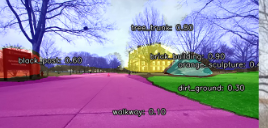
\includegraphics[width=\linewidth,height=38mm,keepaspectratio]{catnav_clipseg.png}
      \end{minipage}\\[0.25em]
      {\scriptsize CLIP Seg}
    \end{column}
    \hfill
    \begin{column}{0.32\textwidth}
      \centering
      \begin{minipage}[t][40mm][c]{\linewidth}
        \centering
        
\includegraphics[width=\linewidth,height=38mm,keepaspectratio]{catnav_costmap_inset.png}
      \end{minipage}\\[0.25em]
      {\scriptsize Cost map}
    \end{column}
    \hfill
    \begin{column}{0.32\textwidth}
      \centering
      \begin{minipage}[t][40mm][c]{\linewidth}
        \centering
        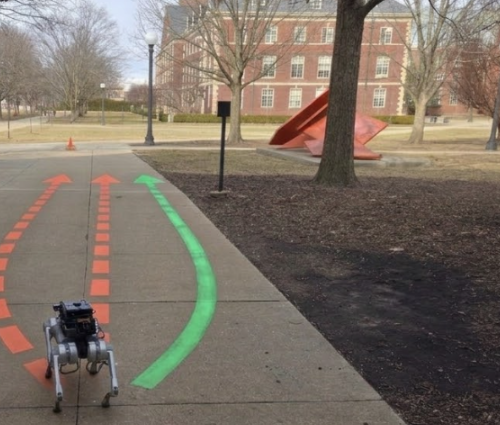
\includegraphics[width=\linewidth,height=38mm,keepaspectratio]{catnav_select.png}
      \end{minipage}\\[0.25em]
      {\scriptsize Select Route}
    \end{column}
  \end{columns}
  \vspace*{0.15em plus 1fill}

  \takeaway{二段階で好みを選ぶ．領域を分け，コストマップを作り，候補経路から一本を選ぶ．}
\end{frame}

\begin{frame}{背景}
  \source{Potnis et al., arXiv, 2026}
  \infocard[gray][20mm]{走破性リスク}{%
    \li ロボットの物理的な能力に対して評価する必要がある
    \li 屋外は動的障害物と地形への配慮
    \li 屋内は人や壊れやすいものへの配慮}
  \vspace{0.7em}
  \begin{columns}[T,onlytextwidth]
    \begin{column}{0.305\textwidth}
      \infocard[orange][24mm]{学習ベース}{%
        \li 大量の学習データが要る
        \li 分布外に弱い}
    \end{column}
    \hfill
    \begin{column}{0.305\textwidth}
      \infocard[blue][24mm]{VLM}{%
        \li コスト化すると柔軟な推論を捨てやすい
        \li 毎回問うと計算が重い}
    \end{column}
    \hfill
    \begin{column}{0.305\textwidth}
      \infocard[green][24mm]{VLA}{%
        \li 速度を直接出せる
        \li なぜその道かを人が読みにくい}
    \end{column}
  \end{columns}

  \takeaway{少ないデータと計算で，数値と人間らしい判断の両方を残したい．}
\end{frame}

\begin{frame}{課題}
  \source{Potnis et al., arXiv, 2026}
  \cardbalance
  \infocard[blue][16mm]{課題 1}{%
    \li 少ないアノテーションでも，高い推論能力が欲しい}
  \vspace{0.28em}
  \infocard[orange][16mm]{課題 2}{%
    \li 少ない計算資源でも，高い周波数で動いてほしい}
  \vspace{0.28em}
  \infocard[green][16mm]{課題 3}{%
    \li 数値だけでなく，社会的で柔軟な判断をしてほしい}
  \takeawaybalance{できれば，その判断が人にとって解釈可能であってほしい．}
\end{frame}

\begin{frame}{貢献}
  \source{Potnis et al., arXiv, 2026}
  \cardbalance
  \infocard[blue][16mm]{貢献 1 ｜ ゼロショットのリスク}{%
    \li タスク固有の学習はせず，VLM の推論で意味的リスク値を推定する}
  \vspace{0.28em}
  \infocard[orange][16mm]{貢献 2 ｜ 評価の再利用}{%
    \li 画像特徴から類似シーンを見つけ，リスク評価をキャッシュして問い合わせを減らす}
  \vspace{0.28em}
  \infocard[green][16mm]{貢献 3 ｜ 経路の選択}{%
    \li RGB に乗せた複数経路から，視覚的に安全な経路を VLM に選ばせる}
  \takeawaybalance{VLM の柔軟な推論を残したまま，必要な問い合わせを減らす．}
\end{frame}

\begin{frame}{方法}
  \source{Potnis et al., arXiv, 2026, Fig.~2}
  \centering
  \begin{tikzpicture}
    \node[inner sep=0] (f) {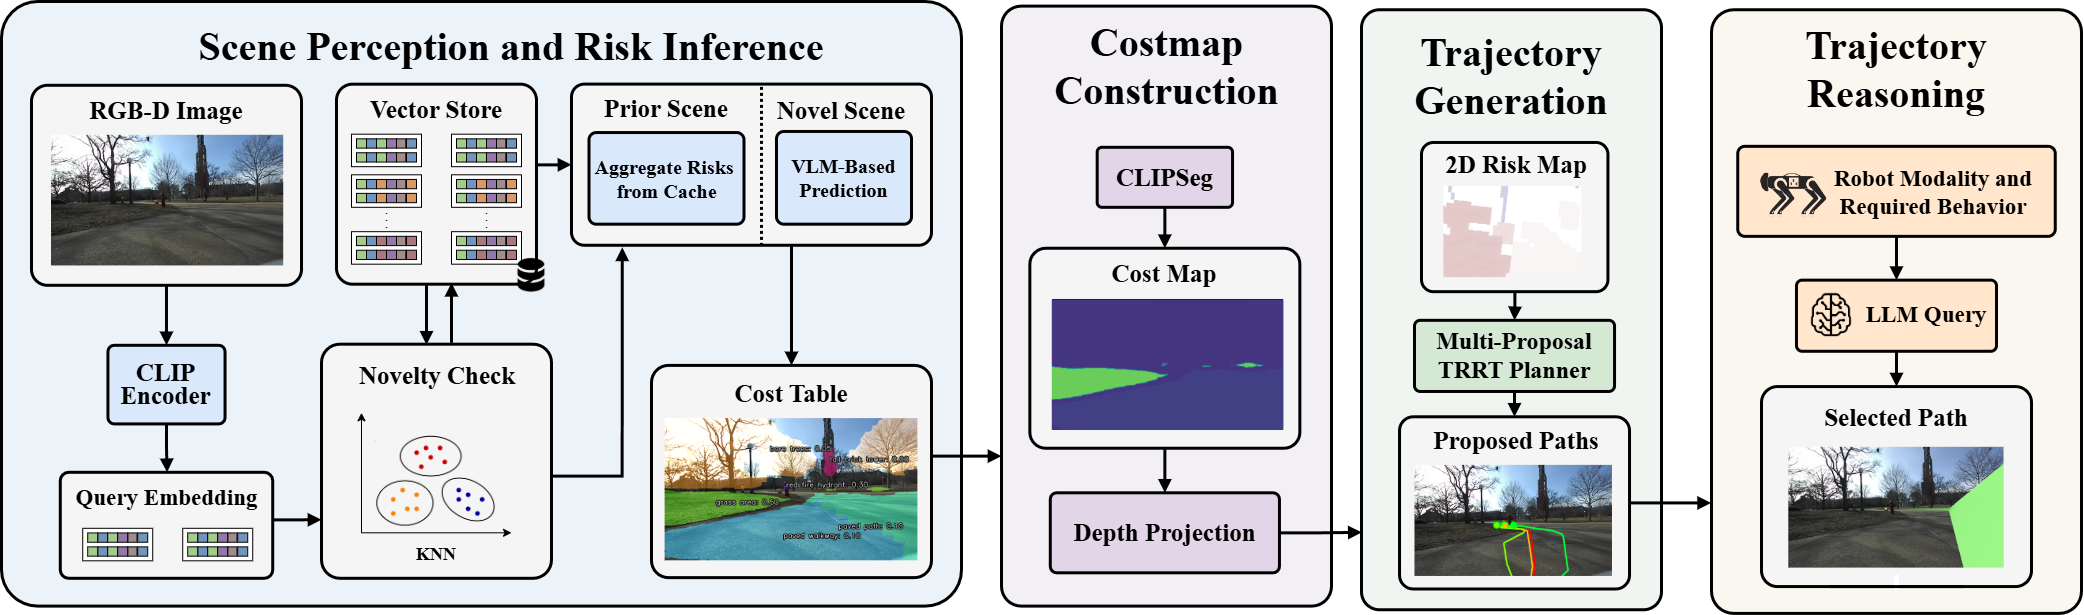
\includegraphics[width=\textwidth,height=40mm,keepaspectratio]{catnav_pipeline.png}};
    \node[anchor=north, font=\scriptsize\bfseries, text=cbluett, align=center]
      at ($(f.south west)!0.24!(f.south east)+(0,-1.6mm)$) {ゼロショット認識};
    \node[anchor=north, font=\scriptsize\bfseries, text=corangett, align=center]
      at ($(f.south west)!0.64!(f.south east)+(0,-1.6mm)$) {リスク数値ベースの\\経路生成};
    \node[anchor=north, font=\scriptsize\bfseries, text=cgreentt, align=center]
      at ($(f.south west)!0.88!(f.south east)+(0,-1.6mm)$) {柔軟な\\経路選択};
  \end{tikzpicture}

  \takeaway{認識，経路生成，経路選択の順で行動が決まる．}
\end{frame}

\begin{frame}{ゼロショット認識}
  \source{Potnis et al., arXiv, 2026}
  \centering
  \scalebox{0.97}{\cacheflow}

  \takeaway{特徴量とコストテーブルはキャッシュに集まり，そこからマップを作る．}
\end{frame}

\begin{frame}{貢献 1 ｜ VLM によるリスク推定}
  \source{Potnis et al., arXiv, 2026}
  \begin{columns}[T,onlytextwidth]
    \begin{column}{0.56\textwidth}
      \infocard[blue][28mm]{コストテーブル}{%
        \li 画像中の物体名と，そのリスクを出させる
        \li タスク用の学習データは使わない
        \li 処理は重く，シーンが新しいときだけ問い合わせる}
      \vspace{0.35em}
      {\footnotesize\color{body}
      コストテーブルは物体名 $c_k$ とリスク $r_k\in[0,1]$ の組．
      \[
        T=\{(c_k,r_k)\}_{k=1}^{K}
      \]}
    \end{column}
    \hfill
    \begin{column}{0.40\textwidth}
      \centering
      \scalebox{0.78}{\cacheflow[vlm]}
    \end{column}
  \end{columns}

  \takeaway{VLM の知識だけでリスクを見積もれるが，毎回は処理したくない．}
\end{frame}

\begin{frame}{貢献 2 ｜ CLIP Encoder ｜ 画像特徴量}
  \source{Potnis et al., arXiv, 2026}
  \begin{columns}[T,onlytextwidth]
    \begin{column}{0.56\textwidth}
      \infocard[blue][22mm]{特徴量}{%
        \li CLIP Encoder で画像を 768 次元の $z_q$ にする
        \li キャッシュ内の特徴量 $z_i$ と距離を比べる}
      \vspace{0.2em}
      {\footnotesize\color{body}
      $\gamma$ は新規性の閾値。最近傍までの距離 $d_{\min}$ が $\gamma$ より大きいシーンだけを新規とみなす。
      \[
        d_{\min}=\min_i\|z_q-z_i\|_2
      \]
      \[
        d_{\min}\le\gamma \;\Rightarrow\; \text{近傍 $k$ 件},\qquad
        d_{\min}>\gamma \;\Rightarrow\; \text{VLM}
      \]}
    \end{column}
    \hfill
    \begin{column}{0.40\textwidth}
      \centering
      \scalebox{0.78}{\cacheflow[clip]}
    \end{column}
  \end{columns}

  \takeaway{画像特徴が近いときは，過去のリスク評価をそのまま使う．}
\end{frame}

\begin{frame}{CLIP-Seg ｜ セグメンテーション}
  \source{Potnis et al., arXiv, 2026}
  \begin{columns}[T,onlytextwidth]
    \begin{column}{0.56\textwidth}
      \infocard[blue][24mm]{反応値}{%
        \li 物体名ラベルとの反応 $p_k(u,v)$ を画素ごとに得る
        \li 最も反応が高い物体を，その画素のクラスにする
        \li 低解像度の反応は，バイリニア補間で画像サイズまで伸ばす}
      \vspace{0.3em}
      {\footnotesize\color{body} ゼロショットのクラス割り当て
      \[
        k^{\star}(u,v)=\arg\max_k p_k(u,v)
      \]}
    \end{column}
    \hfill
    \begin{column}{0.40\textwidth}
      \centering
      \scalebox{0.78}{\cacheflow[seg]}
    \end{column}
  \end{columns}

  \takeaway{物体名との反応の最大値で，ゼロショットにセグメンテーションする．}
\end{frame}

\begin{frame}{CLIP-Seg ｜ コストマップ}
  \source{Potnis et al., arXiv, 2026}
  \begin{columns}[T,onlytextwidth]
    \begin{column}{0.56\textwidth}
      \infocard[blue][20mm]{画素からコストへ}{%
        \li クラスのリスクを画素に乗せてコストマップを作る
        \li 深度を使い，3D から 2D のコストマップへ落とす}
      \vspace{0.25em}
      {\footnotesize\color{body}
      確信度が閾値 $\delta$ を超えた画素だけにリスクを乗せる．
      \[
        M(u,v)=
        \begin{cases}
          r_{k^{\star}} & \text{if } p_{k^{\star}}(u,v)>\delta \\
          0 & \text{otherwise}
        \end{cases}
      \]
      例：舗装 $0.1$，草 $0.3$，人や構造物 $0.7$．}
    \end{column}
    \hfill
    \begin{column}{0.40\textwidth}
      \centering
      \scalebox{0.78}{\cacheflow[map]}
    \end{column}
  \end{columns}

  \takeaway{領域にコストを乗せ，3D から 2D に変換してマップとして使う．}
\end{frame}

\begin{frame}{軌道生成と軌道選択}
  \source{Potnis et al., arXiv, 2026, Fig.~2}
  \begin{columns}[T,onlytextwidth]
    \begin{column}{0.54\textwidth}
      \infocard[orange][10mm]{1．中央}{%
        \li 遷移ベース RRT（T-RRT）で経路を作る}
      \vspace{0.18em}
      \infocard[blue][10mm]{2．左}{%
        \li 中央を，安全条件の範囲で最大 $d$ だけ左へずらす}
      \vspace{0.18em}
      \infocard[green][10mm]{3．右}{%
        \li 中央を，安全条件の範囲で最大 $d$ だけ右へずらす}
      \vspace{0.18em}
      \infocard[violet][10mm]{4．リスク軌道}{%
        \li 安全閾値を緩めた条件で，T-RRT をやり直す}
    \end{column}
    \hfill
    \begin{column}{0.42\textwidth}
      \centering
      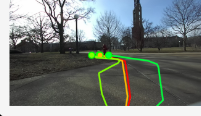
\includegraphics[width=\linewidth]{catnav_paths.png}\\[0.25em]
      {\scriptsize 赤が中央，緑が左右，黄がリスク軌道}
    \end{column}
  \end{columns}

  \takeaway{複数の軌道を作り，VLM に道の種類と安全な理由を考えて選ばせる．}
\end{frame}

\begin{frame}{結果 ｜ VLM によるコスト評価}
  \source{Potnis et al., arXiv, 2026, Fig.~5}
  \centering
  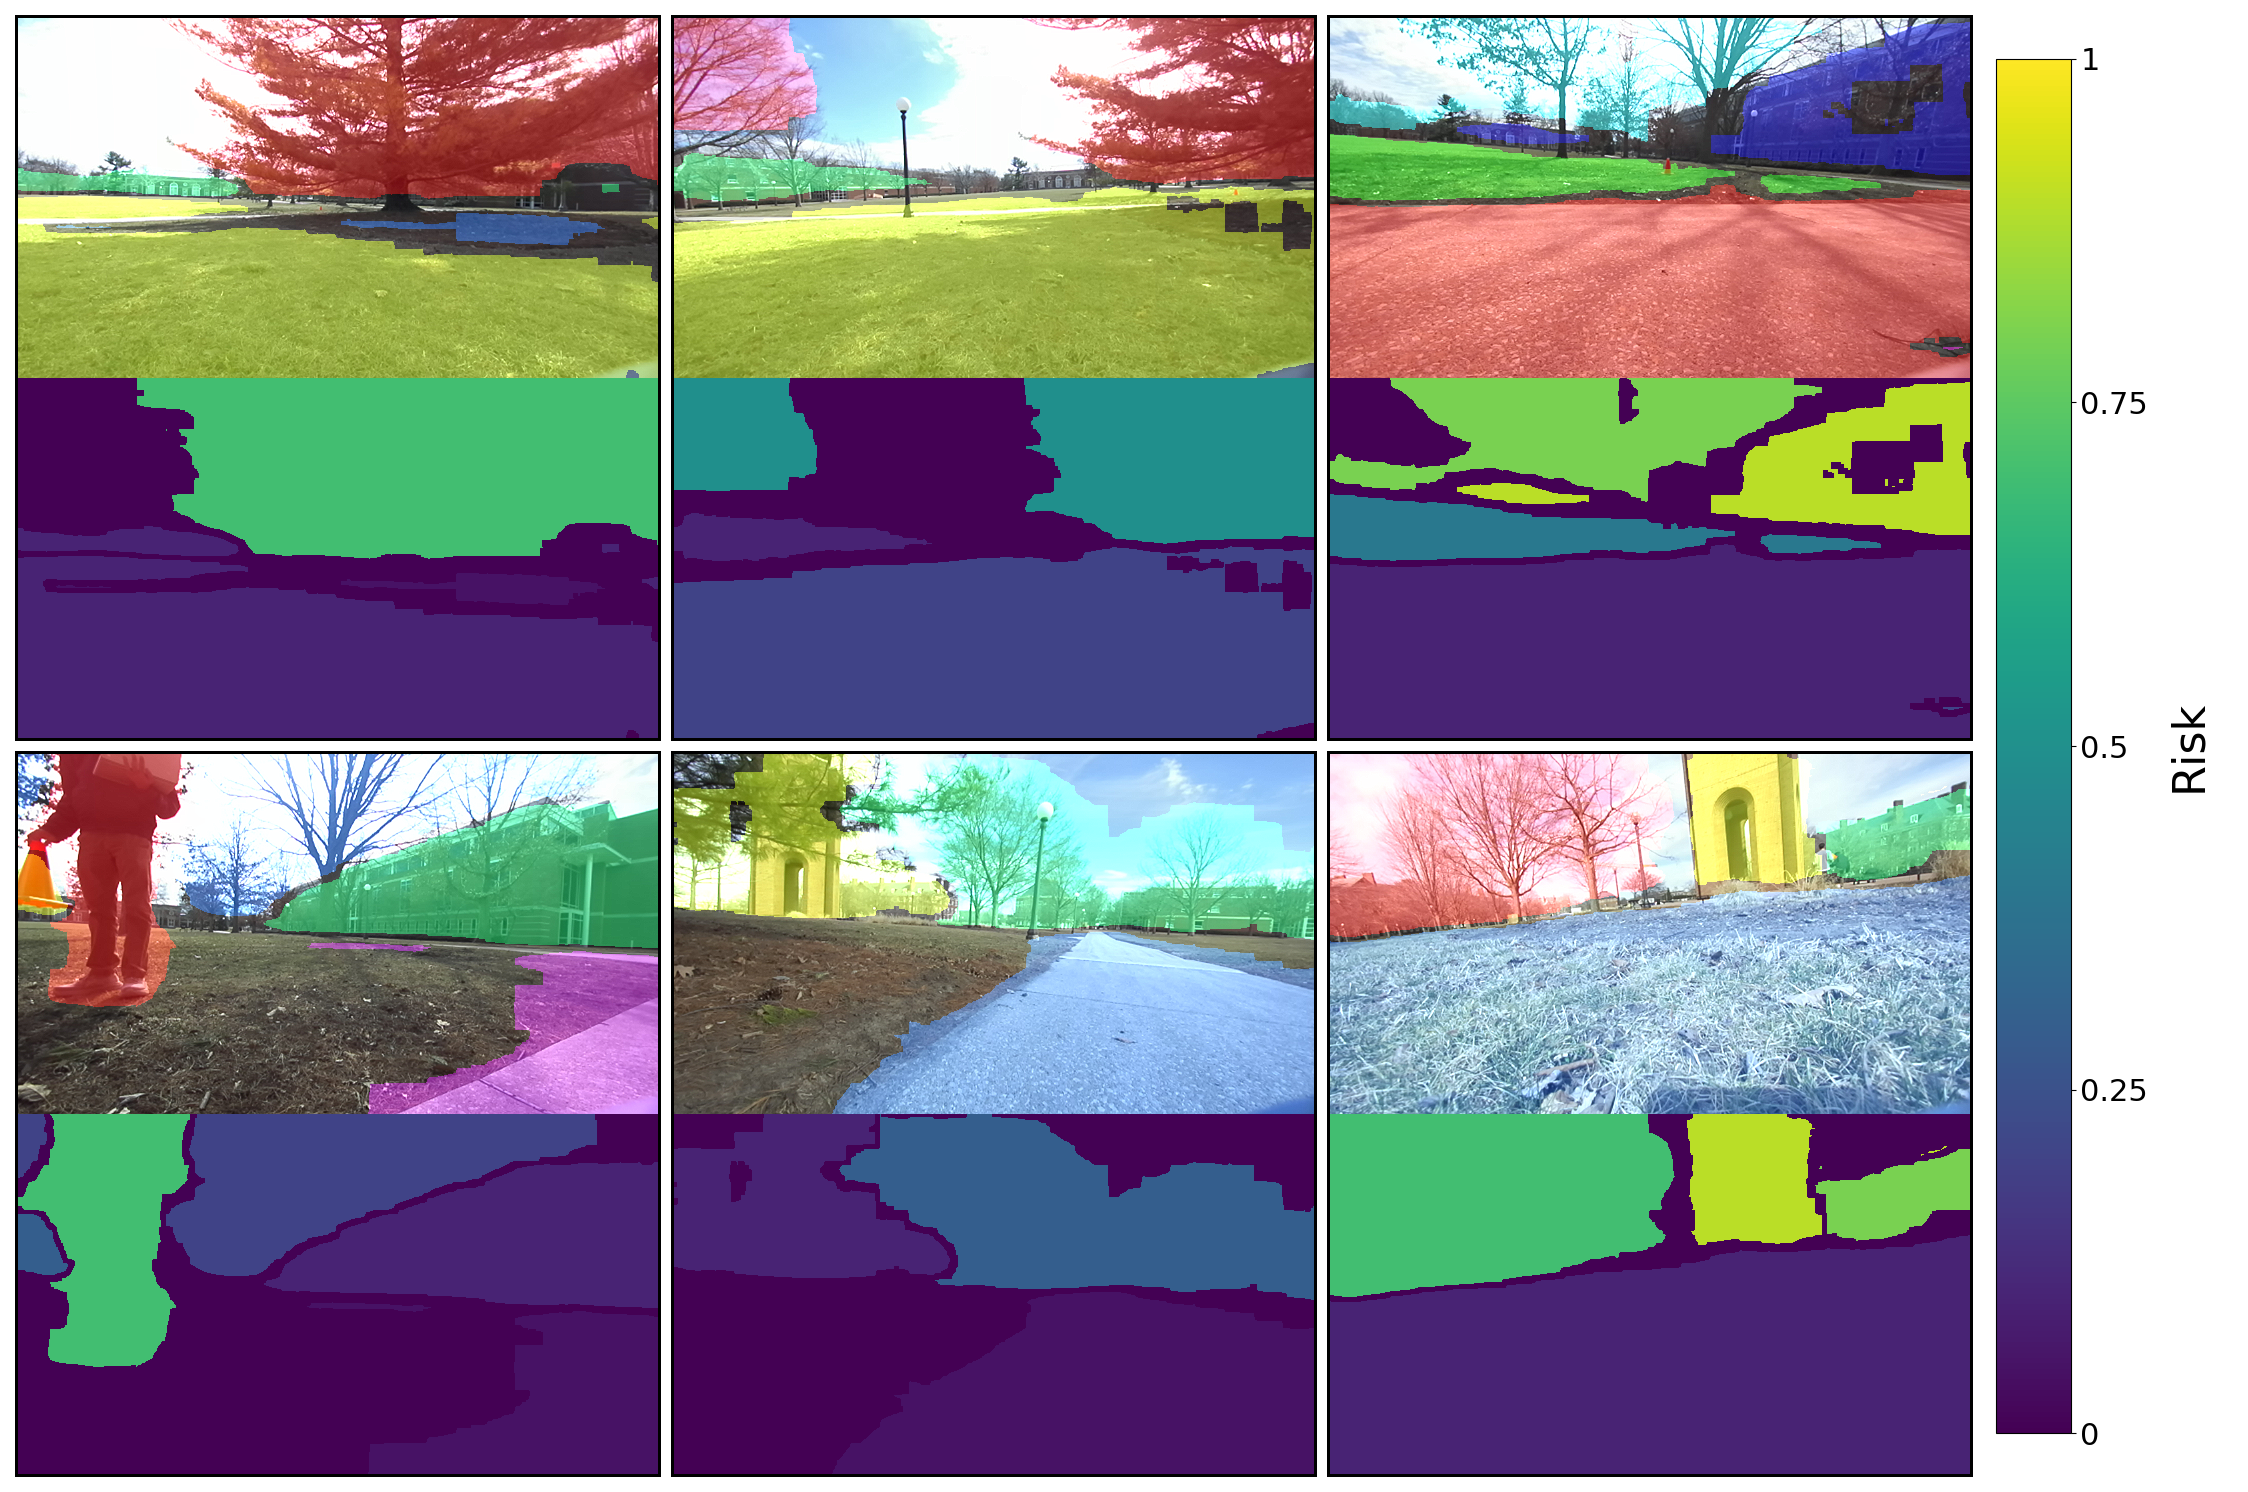
\includegraphics[height=46mm]{catnav_cost.png}

  \vspace{0.15em}
  {\footnotesize 上：セグメンテーション，下：コスト}

  \takeaway{領域ごとにコストが付く．人や構造物はある程度高いリスクになる．}
\end{frame}

\begin{frame}{結果 ｜ VLM への問い合わせ}
  \source{Potnis et al., arXiv, 2026, Table~II}
  \begin{columns}[T,onlytextwidth]
    \begin{column}{0.58\textwidth}
      \centering
      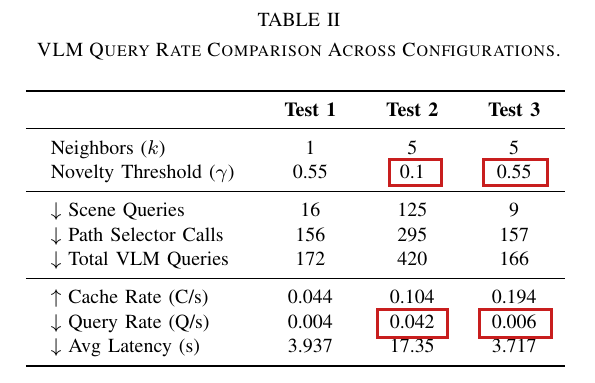
\includegraphics[height=38mm]{catnav_table2.png}
    \end{column}
    \hfill
    \begin{column}{0.40\textwidth}
      \infocard[plain]{実験設定}{%
        \li $k$ はキャッシュから使う近傍の数
        \li $\gamma$ は新規性の閾値。$d_{\min}>\gamma$ だけ VLM に聞く
        \li Test 1 は $k=1$，$\gamma=0.55$
        \li Test 2 は $k=5$，$\gamma=0.1$
        \li Test 3 は $k=5$，$\gamma=0.55$}
      \vspace{0.28em}
      \infocard[orange]{Test 2 と Test 3}{%
        \li Test 2 は $\gamma$ が小さく，多くの画像を新規と判断する
        \li Test 3 は同じ $k=5$ で閾値を戻し，問い合わせを 85.7\% 減らす}
    \end{column}
  \end{columns}

  \takeaway{新規性の閾値を調整すると，画像の問い合わせ回数を減らせる．}
\end{frame}

\begin{frame}{結果 ｜ 柔軟な経路選択}
  \source{Potnis et al., arXiv, 2026, Table~III・Fig.~6}
  \begin{columns}[c,onlytextwidth]
    \begin{column}{0.54\textwidth}
      \centering
      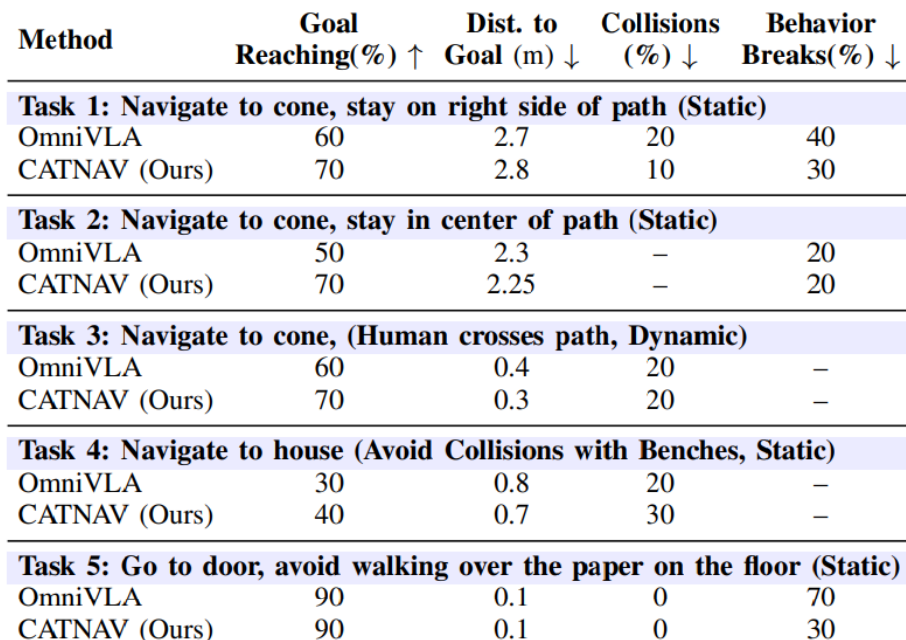
\includegraphics[height=50mm]{survey_table3.png}
    \end{column}
    \hfill
    \begin{column}{0.44\textwidth}
      \centering
      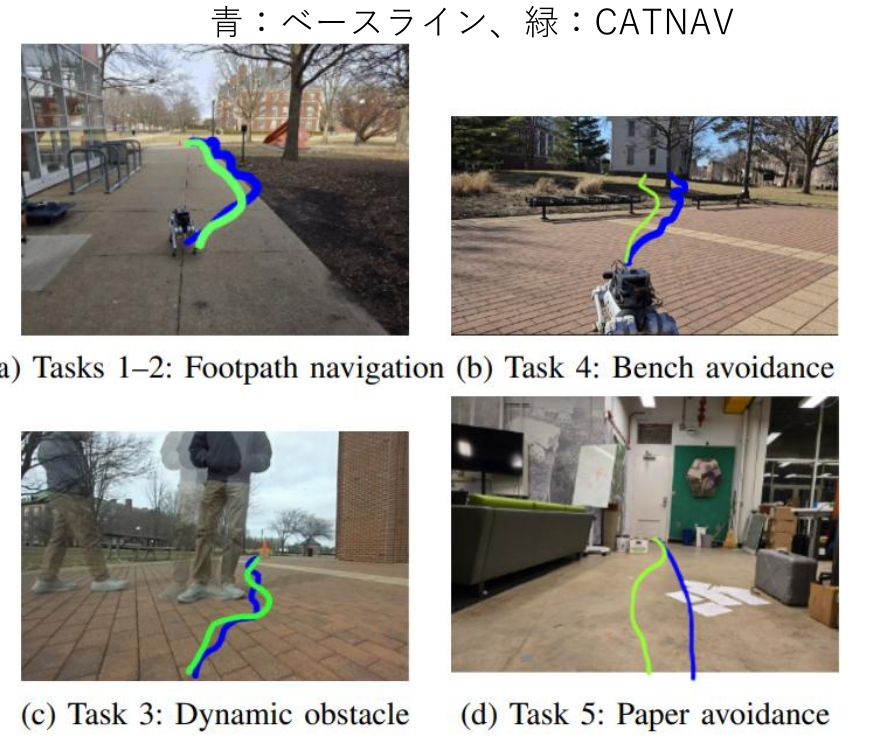
\includegraphics[height=50mm]{survey_trajs.png}
    \end{column}
  \end{columns}

  \takeaway{到達率は平均 68\% 対 58\%．紙をよけるなど，行動違反は 33\% 少ない．}
\end{frame}

\begin{frame}{まとめ ｜ CATNAV}
  \source{Potnis et al., arXiv, 2026}
  \begin{columns}[T,onlytextwidth]
    \begin{column}{0.56\textwidth}
      \infocard[blue][14mm]{貢献 1 ｜ ゼロショットのリスク}{%
        \li タスク学習なしで意味的リスクを推定する．領域ごとにコストが付き，人や構造物は高い}
      \vspace{0.2em}
      \infocard[orange][14mm]{貢献 2 ｜ 評価の再利用}{%
        \li 類似シーンはキャッシュする．Test 3 は Test 2 より VLM 問い合わせを 85.7\% 減らす}
      \vspace{0.2em}
      \infocard[green][14mm]{貢献 3 ｜ 経路の選択}{%
        \li 複数経路から理由つきで一本を選ぶ．到達率は 68\% 対 58\%，行動違反は 33\% 少ない}
    \end{column}
    \hfill
    \begin{column}{0.42\textwidth}
      \infocard[orange][48mm]{リミテーション}{%
        \li 2D--3D 変換でノイズが出る
        \li 軌道の固定パラメータが数か所ある
        \li CLIP-Seg など，ある程度の基盤モデルの能力が要る}
    \end{column}
  \end{columns}

  \takeaway{好みはコストの数値と，見た目による経路選択の二段で表す．}
\end{frame}

% ---------- SEA-Nav ----------

\begin{frame}{SEA-Nav}
  \source{Chen et al., arXiv, 2026}
  \centering
  \acdiagram

  \vspace{0.35em}
  {\footnotesize\color{body}
  通常は Actor の行動を，SEA-Nav は LSE-CBF を通した行動を，Critic が評価する．}

  \takeaway{安全フィルタは後処理ではなく，方策の一部として誤差が伝わる．}
\end{frame}

\begin{frame}{背景}
  \source{Chen et al., arXiv, 2026}
  \infocard[orange][18mm]{自立ナビゲーション}{%
    \li 密な障害物の中の移動は難しく，安全性を上げる必要がある
    \li 大規模な事前学習で，局所環境の性能は上がってきた}
  \vspace{0.3em}
  \infocard[blue][20mm]{安全ナビと CBF}{%
    \li Actor-Critic の外に CBF を置くと，方策は補正されたことを知らない
    \li 失敗でエピソードが終わると，その直前のデータを学習に使いづらい
    \li 取れる失敗サンプルの母数が少ない}

  \takeaway{フィルタの介入も含めて学び，衝突の前後を効率よくサンプルしたい．}
\end{frame}

\begin{frame}{従来手法}
  \source{Chen et al., arXiv, 2026}
  \infocard[gray][18mm]{学習ベースのナビゲーションにおける安全性の担保}{%
    \li 密集した障害物の中でも，衝突せずに進める必要がある
    \li 安全のための介入を，方策自身が学べる必要がある
    \li これまで使われてきたのは，模倣学習，深層強化学習，後処理のフィルタ}
  \vspace{0.55em}
  \begin{columns}[T,onlytextwidth]
    \begin{column}{0.305\textwidth}
      \infocard[orange][22mm]{模倣学習}{%
        \li 行動をまねる
        \li 未知だと失敗しやすい}
    \end{column}
    \hfill
    \begin{column}{0.305\textwidth}
      \infocard[blue][22mm]{深層強化学習}{%
        \li 機動性は出る
        \li 密集すると失敗が多い
        \li 安全制限を掛けにくい}
    \end{column}
    \hfill
    \begin{column}{0.305\textwidth}
      \infocard[green][22mm]{後処理フィルタ}{%
        \li CBF は Actor の外にある
        \li 方策は補正を知らない
        \li 介入を学習できない}
    \end{column}
  \end{columns}

  \takeaway{サンプル効率と，フィルタ込みの安全制御が同時に欲しい．}
\end{frame}

\begin{frame}{貢献}
  \source{Chen et al., arXiv, 2026}
  \cardbalance
  \infocard[blue][16mm]{貢献 1 ｜ End-to-End LSE-CBF}{%
    \li 安全条件を滑らかにし，学習時とテスト時の不一致をなくす}
  \vspace{0.28em}
  \infocard[orange][16mm]{貢献 2 ｜ 運動学的な正則化}{%
    \li 速度の範囲と変化の滑らかさを損失に入れ，実機へ安全に載せる}
  \vspace{0.28em}
  \infocard[green][16mm]{貢献 3 ｜ ACSI}{%
    \li 衝突前後を巻き戻して学び，サンプル効率のボトルネックを減らす}
  \takeawaybalance{安全層・正則化・衝突の再利用の三つで，短い学習でも走破する．}
\end{frame}

\begin{frame}{モデル構造}
  \source{Chen et al., arXiv, 2026, Fig.~2}
  \centering
  \begin{tikzpicture}
    \node[inner sep=0] (fig) {%
      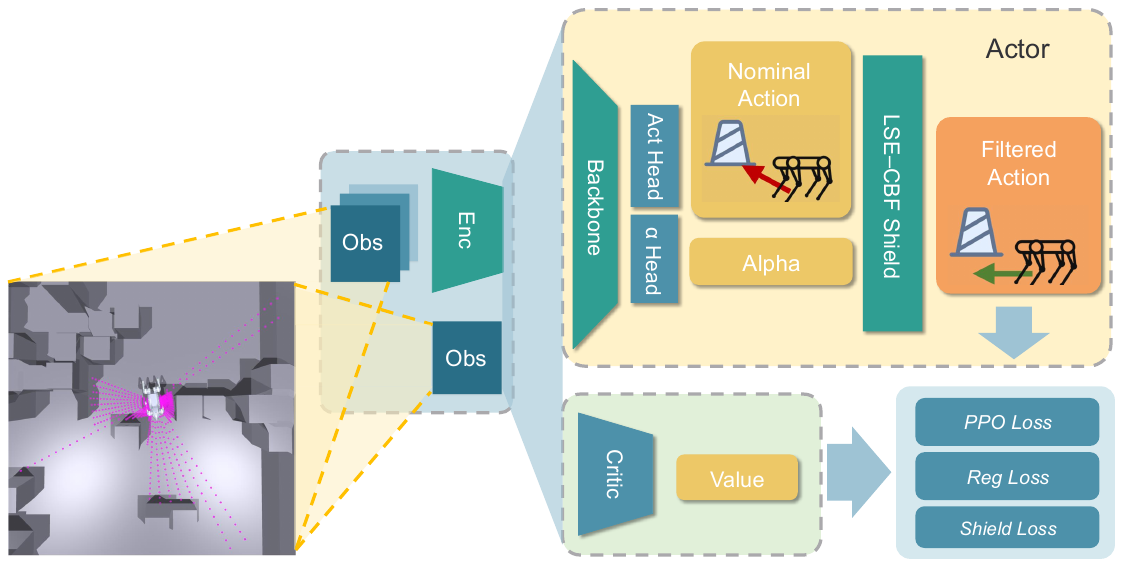
\includegraphics[height=42mm]{seanav_arch.png}};
    \node[anchor=south, font=\scriptsize\bfseries, text=ink]
      at ($(fig.north west)!0.30!(fig.north east)+(0,0.6mm)$) {特徴量抽出};
    \node[anchor=south, font=\scriptsize\bfseries, text=ink]
      at ($(fig.north west)!0.72!(fig.north east)+(0,0.6mm)$) {Actor with CBF};
    \node[anchor=north, font=\scriptsize\bfseries, text=cgreentt]
      at ($(fig.south west)!0.40!(fig.south east)+(0,-0.4mm)$) {Critic};
  \end{tikzpicture}

  \takeaway{Actor は希望速度と $\alpha$ を出し，LSE-CBF を通した速度を損失で学ぶ．}
\end{frame}

\begin{frame}{通常の Actor-Critic との違い}
  \source{Chen et al., arXiv, 2026}
  \centering
  \scalebox{0.86}{\acdiagram}

  \vspace{0.15em}
  \begin{tikzpicture}[x=8mm, y=7mm, font=\scriptsize]
    \node[text=corangett] at (1.3,1.45) {障害物へ向かう};
    \draw[-{Stealth[length=1.6mm]}, draw=corangett, line width=0.75pt] (0.15,0.4) -- (1.85,0.4);
    \draw[fill=corange, draw=corangett] (2.25,0.02) -- (2.7,0.95) -- (3.15,0.02) -- cycle;
    \node[text=muted] at (2.7,-0.28) {障害物};

    \begin{scope}[xshift=52mm]
      \node[text=cgreentt] at (1.5,1.45) {回避できる};
      \draw[-{Stealth[length=1.6mm]}, draw=cgreentt, line width=0.75pt]
        (0.15,0.28) .. controls (1.15,0.28) and (1.2,1.2) .. (2.25,1.05);
      \draw[fill=corange, draw=corangett] (1.85,0.02) -- (2.3,0.95) -- (2.75,0.02) -- cycle;
      \node[text=muted] at (2.3,-0.28) {障害物};
    \end{scope}
  \end{tikzpicture}

  \takeaway{SEA-Nav は，障害物へ向かう行動を CBF で安全範囲へ動かし，その行動を評価する．}
\end{frame}

\begin{frame}{Actor が決める行動}
  \source{Chen et al., arXiv, 2026, Fig.~2}
  \begin{columns}[T,onlytextwidth]
    \begin{column}{0.50\textwidth}
      \infocard[blue][22mm]{入力}{%
        \li 行動履歴 10 フレームの特徴量
        \li 現在の観測
        \lii 41 本のレイで，障害物までの距離}
      \vspace{0.25em}
      \infocard[green][18mm]{出力}{%
        \li 希望する速度指令 $\bar{u}$
        \li CBF の安全制約に関するパラメータ $\alpha$}
    \end{column}
    \hfill
    \begin{column}{0.46\textwidth}
      \centering
      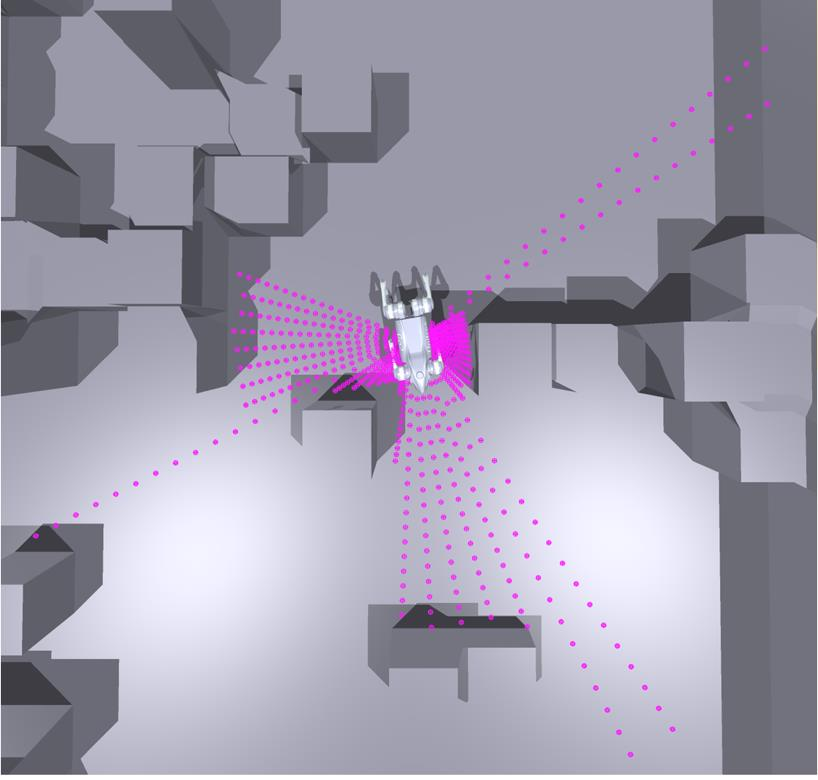
\includegraphics[width=\linewidth,height=42mm,keepaspectratio]{seanav_rays.png}\\[0.15em]
      {\scriptsize ロボットに入力するレイ}
    \end{column}
  \end{columns}

  \takeaway{方策は速度だけでなく，どれだけ安全側に倒すか $\alpha$ も自分で決める．}
\end{frame}

\begin{frame}{貢献 1 ｜ LSE-CBF}
  \source{Chen et al., arXiv, 2026}
  \centering
  各レイに対する安全条件\quad
  $h_i(x)=\rho_i-d_{\mathrm{safe}}$

  \vspace{0.35em}
  \begin{columns}[T,onlytextwidth]
    \begin{column}{0.49\textwidth}
      \infocard[orange][24mm]{通常の CBF}{%
        \centering
        $\displaystyle h(x)=\min_{i\in\{1,\ldots,N\}} h_i(x)$\\[0.25em]
        \raggedright
        \li 最小のレイが入れ替わると不連続
        \li 誤差を流しにくい}
    \end{column}
    \hfill
    \begin{column}{0.49\textwidth}
      \infocard[blue][24mm]{LSE-CBF}{%
        \centering
        {\scriptsize $\displaystyle h(x)=-\frac1k\ln\!\Bigl(\sum_{i=1}^{N}\exp(-k\,h_i(x))\Bigr)$}\\[0.25em]
        \raggedright
        \li 連続なので，悪い指令へ誤差が伝わる}
    \end{column}
  \end{columns}

  \vspace{0.35em}
  \centering
  CBF の安全制約 $\dot h(x,u)\ge -\alpha h(x)$ にしたがい，\\
  入力を安全な範囲へ最小限動かす．
  \[
    \min_{u_s}\tfrac12\|u_s-\bar{u}(x)\|^2
    \quad\text{s.t.}\quad
    \langle L_g h(x), u_s\rangle+\alpha h(x)\ge 0
  \]

  \takeaway{通常の最小値は不連続で，LSE は連続なので誤差が伝わる．}
\end{frame}

\begin{frame}{貢献 2 ｜ 損失関数}
  \source{Chen et al., arXiv, 2026}
  \vspace{-0.35em}
  \[
    L_{\mathrm{total}}=L_{\mathrm{PPO}}+\lambda_{\mathrm{shield}}L_{\mathrm{shield}}+\lambda_{\mathrm{reg}}L_{\mathrm{reg}}
  \]
  \vspace{-0.9em}
  \begin{columns}[T,onlytextwidth]
    \begin{column}{0.46\textwidth}
      \infocard[blue][16mm]{$L_{\mathrm{PPO}}$}{%
        \li 方策を更新する損失
        \li 行動の良し悪しは，Critic の評価から学ぶ}
      \vspace{0.22em}
      \infocard[orange][22mm]{$L_{\mathrm{shield}}$}{%
        \li フィルタの動かしすぎと，$\alpha$ の不足を避ける
        \li {\scriptsize $L_{\mathrm{shield}}=\|u_{s,t}-\bar{u}_t\|^2+[\alpha_{\min}-\alpha_t]_{+}^{2}$}}
    \end{column}
    \hfill
    \begin{column}{0.52\textwidth}
      \infocard[green][42mm]{$L_{\mathrm{reg}}$　運動学}{%
        \li 二つの項の和。$L_{\mathrm{reg}}=L_{\mathrm{range}}+L_{\mathrm{smooth}}$
        \li 速度の上限
        \li {\scriptsize $L_{\mathrm{range}}=\sum_{j\in\{x,y,\omega\}}\bigl(u_{s,t}^{j}-\mathrm{clip}(u_{s,t}^{j},u_{j}^{\min},u_{j}^{\max})\bigr)^{2}$}
        \li 方針の急変を抑える
        \li {\scriptsize $L_{\mathrm{smooth}}=\lambda_{\pi} D(\pi_{\theta}(x_t),\pi_{\theta}(\bar{x}_t))+\lambda_{V} D(V_{\phi}(x_t),V_{\phi}(\bar{x}_t))$}}
    \end{column}
  \end{columns}

  \takeaway{正則化により，実機で安全かつ滑らかな速度指令を出せる．}
\end{frame}

\begin{frame}{貢献 3 ｜ ACSI}
  \source{Chen et al., arXiv, 2026}
  {\footnotesize\color{body}
  バッファには直近 2 秒，100 ステップを保存する．衝突したあとには大きなペナルティを与える．}

  \vspace{0.55em}
  \begin{columns}[T,onlytextwidth]
    \begin{column}{0.49\textwidth}
      \infocard[orange][18mm]{早期終了}{%
        \li $P_{\mathrm{reset}}$ でエピソードを打ち切り，次へ進む}
    \end{column}
    \hfill
    \begin{column}{0.49\textwidth}
      \infocard[blue][18mm]{巻き戻し}{%
        \li $P_{\mathrm{replay}}$ で 2 秒戻り，回避をやり直す}
    \end{column}
  \end{columns}

  \vspace{0.4em}
  {\color{body} リセット率はゴール率に合わせて変える．}
  \[
    P_{\mathrm{reset}}=P_{\min}+(P_{\max}-P_{\min})\cdot\mathrm{clip}(L_{\mathrm{goal}}/1.5,\,0,\,1)
  \]

  \takeaway{衝突した履歴を効率よく引くので，危険な局所を重点的に学べる．}
\end{frame}

\begin{frame}{結果 ｜ シミュレーション}
  \source{Chen et al., arXiv, 2026, Table~I}
  \centering
  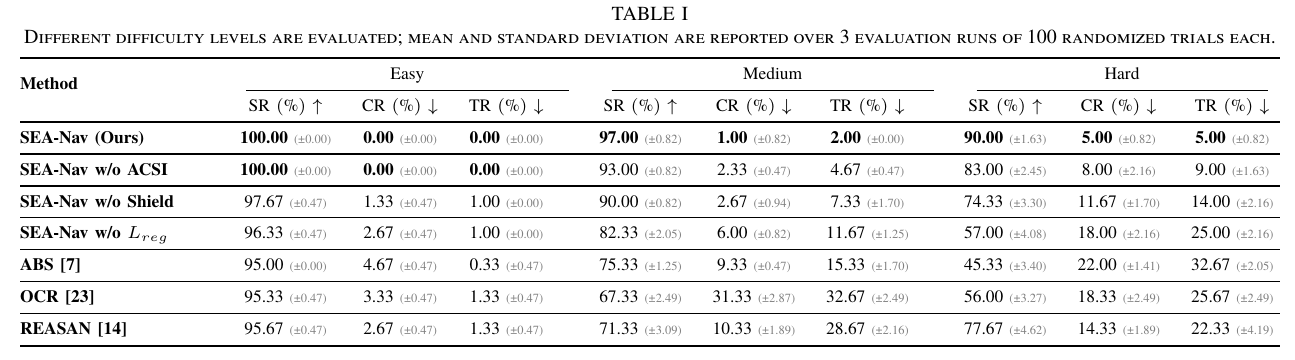
\includegraphics[width=\textwidth]{seanav_table1.png}

  \vspace{0.3em}
  {\scriptsize\color{body}
  RTX 4090 で 2000 iteration，約 1 時間．10\,m 四方．SR は成功率，CR は衝突率，TR は時間切れ．\\
  Hard の衝突率は，SEA-Nav が 5\%，ACSI なしが 8\%，Shield なしが約 12\%，$L_{\mathrm{reg}}$ なしが 18\%．}

  \takeaway{寄与は Easy では小さく，障害物が密な Hard で差が開く．}
\end{frame}

\begin{frame}{結果 ｜ 実機}
  \source{Chen et al., arXiv, 2026, Table~II・Fig.~5．Unitree Go2}
  \centering
  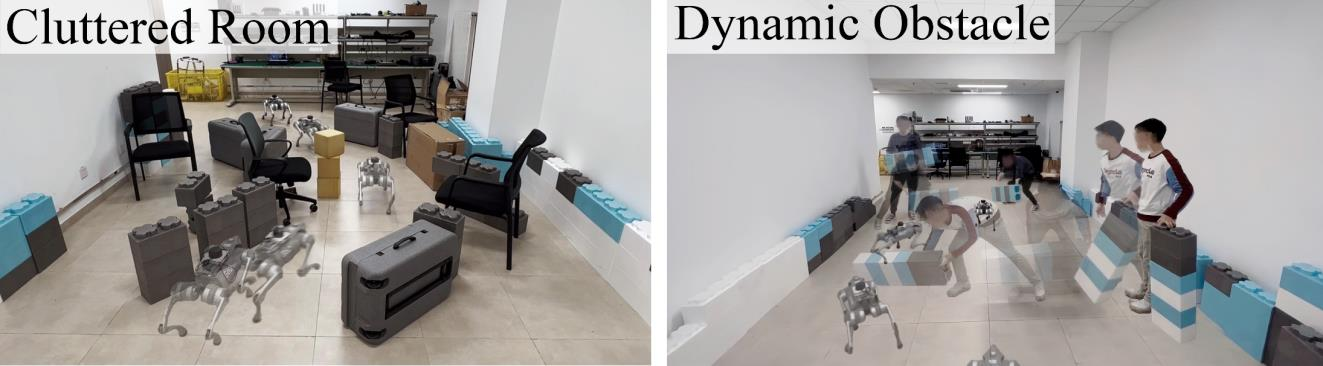
\includegraphics[width=0.49\textwidth,height=16mm,keepaspectratio]{seanav_real_ab.png}\hfill
  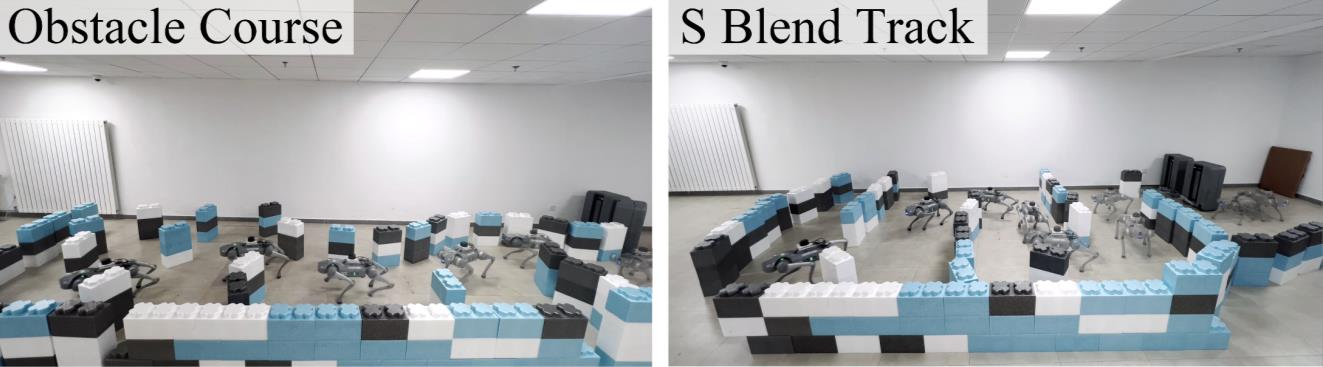
\includegraphics[width=0.49\textwidth,height=16mm,keepaspectratio]{seanav_real_cd.png}

  \vspace{0.2em}
  {\scriptsize\color{body}
  SEA-Nav は学習した歩行モデル，SEA-Nav-b は Unitree 公式の歩行モデル．}

  \vspace{0.15em}
  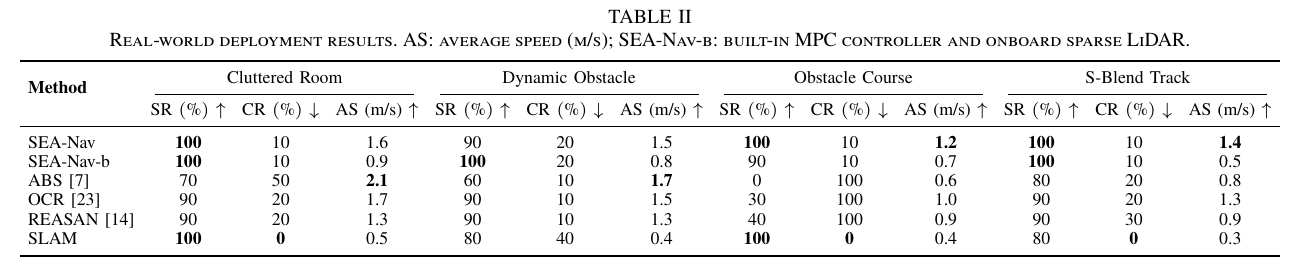
\includegraphics[width=\textwidth]{seanav_table2.png}

  \takeaway{4 環境の多くで SEA-Nav の成功率が高く，公式モデルや SLAM より速い．}
\end{frame}

\begin{frame}{まとめ ｜ SEA-Nav}
  \source{Chen et al., arXiv, 2026}
  \begin{columns}[T,onlytextwidth]
    \begin{column}{0.58\textwidth}
      \infocard[blue][15mm]{貢献 1 ｜ End-to-End LSE-CBF}{%
        \li 安全条件を滑らかにし，学習と実行の安全層を一致させる．Hard の成功率は 90\%}
      \vspace{0.2em}
      \infocard[orange][15mm]{貢献 2 ｜ 運動学的な正則化}{%
        \li 速度の範囲と変化の滑らかさを損失に入れる．実機では 1.2--1.6\,m/s で走る}
      \vspace{0.2em}
      \infocard[green][15mm]{貢献 3 ｜ ACSI}{%
        \li 衝突前後を巻き戻して学ぶ．Hard の衝突率は 5\% まで下がる}
    \end{column}
    \hfill
    \begin{column}{0.40\textwidth}
      \infocard[orange][48mm]{リミテーション}{%
        \li フラットな路面を想定している
        \li 複雑な行き止まりは未対応}
    \end{column}
  \end{columns}

  \takeaway{安全は速度指令を通す微分可能な制約として入る．}
\end{frame}

\begin{frame}{まとめ ｜ 2本のサーベイ}
  \cardbalance
  \begin{columns}[T,onlytextwidth]
    \begin{column}{0.49\textwidth}
      \infocard[green][48mm]{CATNAV ｜ 好み}{%
        \li VLM が意味的なリスクをゼロショットで付ける
        \li 似た画像はキャッシュし，問い合わせを減らす
        \li 複数経路を見て，指示に合う一本を選ぶ
        \li 歩き方の好みは，経路選択の理由として入る}
    \end{column}
    \hfill
    \begin{column}{0.49\textwidth}
      \infocard[blue][48mm]{SEA-Nav ｜ 安全}{%
        \li レイの距離から，安全な速度指令を直接学ぶ
        \li CBF は後処理ではなく，評価と損失に入る
        \li 衝突の巻き戻しで，密集環境を短時間で学ぶ
        \li 安全保障は，速度の制約として入る}
    \end{column}
  \end{columns}
  \takeawaybalance{好みは経路の選択，安全は速度の制約．局所プランナではこの二つを重ねたい．}
\end{frame}

\end{document}
